\section{Mines and Specifications}

\subsection{What is a landmine}

\begin{wrapfigure}{R}{0.47\linewidth}
\centering
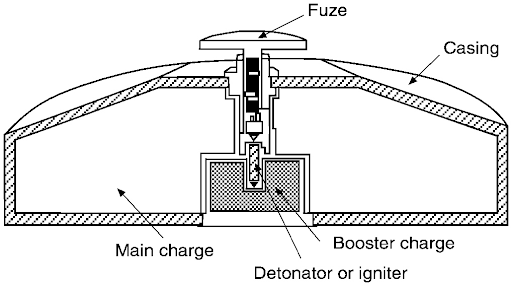
\includegraphics[width=\linewidth]{00 - Images/composition of vehicle landmine.png}
  \caption{Composition of Vehicle Landmine \cite{NAP10071}}
  \label{fig:composition of vehicle landmine}
\end{wrapfigure}

Landmines are explosive devices with an unmanned trigger mechanism. Landmines are constructed with the specific needs to either disable vehicles or personnel. The content of mines varies based on target area, but all mines have a trigger mechanism and a main explosive charge. Mines usually consist of an explosive chain reaction being initiated by the trigger mechanism. As in the case with figure xx2 the chronological order of initiation is the fuse then the detonator or ignited followed by the booster charge and finally the main charge. Landmines have different shapes and sizes based on their intended target. anti-personnel mines are usually small

\subsection{Explosions and pressure waves}

Explosive material is overall but into two types; low and high explosive. A low explosive material creates a pressure wave with enough force to push/move objects possibly at great velocity. High explosive material creates shockwaves that potentially crush objects at relatively close proximity (to the detonation) while pushing away anything in its radius. Low or high explosive refers to the burn rate of material. A pressure wave from an exploding landmine is usually created by expanding gasses released from the combustion of the main charge. This wave of pressurized gasses travels outwards from the explosion in all directions with its highest velocity in the beginning and then fast decelerates over the distance. At some point the wave moves backwards to fill out the vacuum created by the explosion at the origin point of the wave \cite{Siegelbook}.

\subsection{Landmines, their Placement and Trigger Mechanisms}

For an anti-personnel landmine to be effective against its subject  
For landmines to be effective against “enemy” forces they have to be hidden out of sight while close enough for its detonation to release a critical force upon the target/subject. Often range from 60-140 mm in diameter. \textbf{Anti-personnel} mines have two main ways of injuring the subjects;
\begin{enumerate}
    \item The force of the shock-wave crushing and “throwing” away the subject.
    \item The casing of the mine and its surrounding is accelerated in all directions by the explosion, penetrating objects in a large area
\end{enumerate}

\begin{wrapfigure}{R}{0.47\linewidth}
\centering
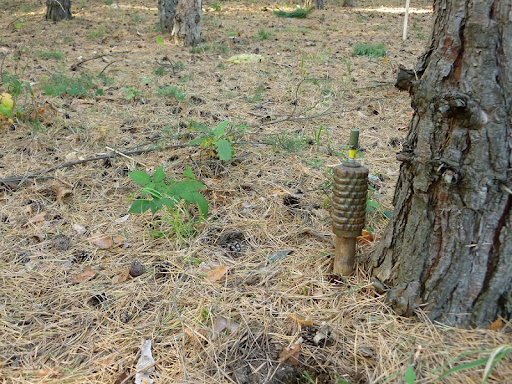
\includegraphics[width=\linewidth]{00 - Images/evolution-landmines-to-ieds.png}
  \caption{An AP Stake Mine with tripwire, Kosovo \cite{LinternWebsite}}
  \label{fig:An AP Stake Mine with tripwire, Kosovo}
\end{wrapfigure}
Mines meant to crush the victim with the pure force of the shock-wave has to be placed in close proximity to the target. One way to compensate for the distance is sizing up the explosive charge for a greater blast radius. The trigger mechanism for this type of mine is usually part of the casing of the mine, meaning the victim/target is required to disturb the mine directly. The most common trigger mechanism here is in integrated presurplate built into the mine requiring the victim/target to step on or possibly just close to it depending on the trigger’s sensitivity. The other type of anti-personnel landmines are \textbf{pre fragmented landmines} placed on or possibly over the ground with the main effect on victims being fragments of the outer casing and (as well as) the surrounding. The advantage here is a larger area of effect while the downside is the mine and the tripwire being visible as seen on figure \ref{fig:An AP Stake Mine with tripwire, Kosovo}. \textbf{Anti-vehicle} mines usually range from 1 - 20 kg and either target the wheels, control device and engine or the “belly” of the vehicle. 

%\section{One specific landmine:}
%The name, functionality and specifications/stats.

\subsection{Landmines in Warfare}

Deploying landmines in conventional warfare has been done in a wide variety of ways over the time. The most common is minefields laid by hand and usually mapped by combat engineers to make the removal of it more convenient. These landmines usually get hidden in the ground and they can be a combination of anti-personnel and anti-vehicle mines. It depends entirely on whether or not the armed forces have the capacity and the will to do so. In war it is not always possible to make an accurate map over the deployed mines location. Sometimes it comes down to the time required while other times it depends on the method of deployment e.g. with usage of cluster munition from artillery and aircrafts to deliver multiple mines at a time and even as an offencive do to the long range. With this method it is nearly impossible to make an accurate map of the newly deployed minefield as well as marking the minefield. Although they will be visible at first, they will end up blending in with nature over time and as years pass they may sink into the ground. In \textbf{conventional warfare} these fast but nearly impossible to map methods are often avoided because of their harmful effect on the land during and even after the war/conflict. A common use of landmines are minefields made with the purpose of leading the enemy forces into an disadvantageous position in the terrain, allowing friendly troops to take a favorable position turning it into a battlefield. This is all part of a defensive maneuver where the enemy has to choose between moving through the minefield or possible into an ambush. When preparing an ambush the defending army will choose an advantageous position, usually some sort of high ground. Then place or prepare an obstacle with the purpose of bringing the enemy to a full stop. When that happens the introding force would be taken under fire and forced to either push through the obstacle or fall back. Such obstacles could be large objects on the road blocking passage or barbed wire. It would likely be reinforced by numerous landmines to make the removal even more difficult and time consuming. At this point the attacking force would be desperate to breach through to the obstacle, possibly using explosives to speed up the process. Doing this mine from around the obstacle would be displaced and the entire maneuver would make it extremely difficult to find the landmines afterwards.

\subsection{Landmines in Conflict Zones}

For unconventional warfare there are no rules and thereby almost nothing to protect civilians as well as the land from being “affected” more than necessary by the conflict. In this chase it is unlikely that the unconventional force has access to mass production of landmines and therefore makes use of improvised solutions. This could involve re-purposing other types of munition into creative but unorthodox landmines and explosive devices also known as improvised explosive devices (IED).\\

\iffalse
\section*{All Sources in this Section}

Historical use of mines:\\ https://onlinelibrary-wiley-com.zorac.aub.aau.dk/doi/10.1002/9781444338232.wbeow414

\vspace{2mm}

Blast injuries:\\ https://tbi.cemmlibrary.org/Moderate-to-Severe-TBI/Mechanisms-of-TBI/Blast-Injuries 

\vspace{2mm}

Chemistry in explosions:\\ https://ebookcentral.proquest.com/lib/aalborguniv-ebooks/reader.action?docID=4182981&ppg=236 

\vspace{2mm}


Evolution landmines to IEDs:\\ https://neillintern.com/2017/12/15/evolution-landmines-to-ieds/ 

\vspace{2mm}

What is landmines:\\ https://www.nap.edu/read/10071/chapter/5#27 

\vspace{2mm}

Landmines and mine action:\\ http://web.mit.edu/demining/assignments/understanding-landmines.pdf 

\vspace{2mm}

Facts about landmines:\\ https://www.landminefree.org/2017/index.php/support/facts-about-landmines 

There has only been used sources from the above sources.
\fi


\iffalse
Mines are usually simple mechanisms that commonly consist of a container, the internal explosive material, and a trigger. These components can vary according to their intended purpose or accessibility \cite{LandmineDetectionTechniques2010}.


The container can be made with a variety of different materials, ex. plastic, wood, metal, or a combination of those three \cite{LandmineDetectionTechniques2010}. This raises a problem for the mine detection techniques since the materials and size of the explosive device can vary a lot. Improvised mines are usually made with materials available at hand \cite{DetectionAndLocalizationOfImprovisedDevices2010}. That includes both the casing, the explosive material, and the trigger. The trigger component is what will detonate the mine. The mine could be activated by an electronic or pressure sensor. If the mine is intended as an anti-personnel mine with a pressure sensor, then it usually requires a pressure between 5-16 kg to initiate. Anti-tank mines require more than 100kg pressure to initiate. Some mines are buried just below the ground while others have their triggers above the ground \cite{LandmineDetectionTechniques2010}.


The most common purpose of landmines and unexploded ordnance (UXO) is not necessarily to kill the victim, but to disable personnel and/or equipment. This can result in long-term medical and psychological trauma, as well as being a financial burden for the affected individuals. As well as the mine action, see Figure \ref{fig:contributions_by_thematic_sector_2018}. Areas covered in mines can restrict access to clean water, arable land, roads, healthcare services, and facilities \cite{OxfordAcademic2005}. Therefore, it is easy to see the benefits that can be gained from demining. 
\fi